\documentclass{beamer}

\mode<presentation>
{
  \usetheme{default}
  \usecolortheme{default}
  \usefonttheme{default}
  \setbeamertemplate{navigation symbols}{}
  \setbeamertemplate{caption}[numbered]
  \setbeamertemplate{footline}[page number]
  \setbeamercolor{frametitle}{fg=white}
  \setbeamercolor{footline}{fg=black}
} 

\usepackage[english]{babel}
\usepackage[utf8x]{inputenc}
\usepackage{tikz}
\usepackage{listings}
\usepackage{courier}
\usepackage{array}
\usepackage{bold-extra}
\usepackage{minted}

\xdefinecolor{darkblue}{rgb}{0.1,0.1,0.7}
\xdefinecolor{darkgreen}{rgb}{0,0.5,0}
\xdefinecolor{darkgrey}{rgb}{0.35,0.35,0.35}
\xdefinecolor{darkorange}{rgb}{0.8,0.5,0}
\xdefinecolor{darkred}{rgb}{0.7,0,0}
\xdefinecolor{dianablue}{rgb}{0.18,0.24,0.31}
\definecolor{commentgreen}{rgb}{0,0.6,0}
\definecolor{stringmauve}{rgb}{0.58,0,0.82}

\lstset{ %
  backgroundcolor=\color{white},      % choose the background color
  basicstyle=\ttfamily\small,         % size of fonts used for the code
  breaklines=true,                    % automatic line breaking only at whitespace
  captionpos=b,                       % sets the caption-position to bottom
  commentstyle=\color{commentgreen},  % comment style
  escapeinside={\%*}{*)},             % if you want to add LaTeX within your code
  keywordstyle=\color{blue},          % keyword style
  stringstyle=\color{stringmauve},    % string literal style
  showstringspaces=false,
  showlines=true
}

\lstdefinelanguage{scala}{
  morekeywords={abstract,case,catch,class,def,%
    do,else,extends,false,final,finally,%
    for,if,implicit,import,match,mixin,%
    new,null,object,override,package,%
    private,protected,requires,return,sealed,%
    super,this,throw,trait,true,try,%
    type,val,var,while,with,yield},
  otherkeywords={=>,<-,<\%,<:,>:,\#,@},
  sensitive=true,
  morecomment=[l]{//},
  morecomment=[n]{/*}{*/},
  morestring=[b]",
  morestring=[b]',
  morestring=[b]"""
}

\title[2017-06-01-threadsafe-histograms]{Thread-safe histograms}
\author{Jim Pivarski}
\institute{Princeton University -- DIANA}
\date{June 1, 2017}

\begin{document}

\logo{\pgfputat{\pgfxy(0.11, 8)}{\pgfbox[right,base]{\tikz{\filldraw[fill=dianablue, draw=none] (0 cm, 0 cm) rectangle (50 cm, 1 cm);}}}\pgfputat{\pgfxy(0.11, -0.6)}{\pgfbox[right,base]{\tikz{\filldraw[fill=dianablue, draw=none] (0 cm, 0 cm) rectangle (50 cm, 1 cm);}
\includegraphics[height=0.99 cm]{diana-hep-logo.png}\tikz{\filldraw[fill=dianablue, draw=none] (0 cm, 0 cm) rectangle (4.9 cm, 1 cm);}}}}

\begin{frame}
  \titlepage
\end{frame}

\logo{\pgfputat{\pgfxy(0.11, 8)}{\pgfbox[right,base]{\tikz{\filldraw[fill=dianablue, draw=none] (0 cm, 0 cm) rectangle (50 cm, 1 cm);}
\includegraphics[height=1 cm]{diana-hep-logo.png}}}}

% Uncomment these lines for an automatically generated outline.
%\begin{frame}{Outline}
%  \tableofcontents
%\end{frame}

%%%%%%%%%%%%%%%%%%%%%%%%%%%%%%%%%%%%%%%%%%%%%%%%%%%%%%%

\begin{frame}{Overheard at a CMS Core meeting:}

\Large DAQ makes thousands of histograms.

\vspace{0.5 cm}
To safely fill them in parallel threads, they're scattered into thread-local copies, gathered by hsitogram-addition.

\vspace{0.5 cm}
But this uses so much working memory, some tasks can't be performed.
\end{frame}

\begin{frame}{So I wondered\ldots}

\begin{center}
\LARGE What is the cost of a thread-safe histogram?
\end{center}
\end{frame}

\begin{frame}{How could it be implemented?}
\large
\begin{description}
\item[Idea \#1:] make each histogram an actor with a thread-safe queue as a mailbox. ``Fill'' sends a message.
\end{description}

\uncover<2->{\small\textcolor{darkgreen}{No. These things work when load is variable, allowing the receiver to catch up on old messages during low load without slowing down the sender. Doing this in a steady-load environment doesn't make sense.}\large}

\begin{description}
\item[Idea \#2:] block write access at the granularity of {\it bins.}
\end{description}

\textcolor{darkblue}{\hspace{1.5 cm}using locks?}

\uncover<3->{\small\textcolor{darkgreen}{No. The memory overhead of a lock per bin would defeat the purpose (saving memory), and a lock per histogram is too coarse.}\large}

\vspace{0.2 cm}
\textcolor{darkblue}{\hspace{1.5 cm}compare-and-swap?}

\uncover<4->{\small\textcolor{darkgreen}{Sounds good: per-bin contention is low and the work to be repeated in the case of a collision is minimal. No extra memory required.}\large}

\vspace{0.2 cm}
\textcolor{darkblue}{\hspace{1.5 cm}{\tt std::atomic}?}

\uncover<5->{\small\textcolor{darkgreen}{I originally thought this did locking, but I was wrong.}\large}
\end{frame}

\begin{frame}[fragile]{\only<1>{Naive implementation: unsafe baseline}\only<2>{Compare-and-swap implementation}\only<3>{{\tt std::atomic} implementation}}
\vspace{0.5 cm}
Python script sets up many threads, feeds them all the {\it same} block of memory ({\tt\small fillme}), and starts them all at the same time.

\vspace{0.25 cm}
\tiny
\begin{minted}{c++}
double fill(long *fillme, long size, long trials, long cardinality, long *collisions) {
  struct timeval startTime, endTime;
  int shift = (int)floor(log2((double)size / cardinality));   // control collision rate
\end{minted}
\begin{onlyenv}<3>
\begin{minted}[frame=single]{c++}
  // reinterpret the block of memory as an array of atomics
  std::atomic<long>* fillme2 = reinterpret_cast<std::atomic<long>*>(fillme);
\end{minted}
\end{onlyenv}
\begin{minted}{c++}
  std::mt19937 rng;                              // thread-local random number generator
  rng.seed(std::random_device()());
  std::uniform_int_distribution<long> distribution(0, cardinality - 1);

  gettimeofday(&startTime, 0);                   // start the stopwatch
  for (long i = 0;  i < trials;  i++) {
    long value = distribution(rng) << shift;     // drop LSBs to get more collisions
\end{minted}
\begin{onlyenv}<1>
\begin{minted}[frame=single]{c++}
    fillme[value]++;                             // naive increment bin
\end{minted}
\end{onlyenv}
\begin{onlyenv}<2>
\begin{minted}[frame=single]{c++}
    long *ptr = &fillme[value];
    long oldval = *ptr;                          // try...
    long newval = oldval + 1;
    while (CAS(ptr, oldval, newval) != oldval) {
      oldval = *ptr;                             // ...try again
      newval = oldval + 1;
      (*collisions)++;                           // measure actual collision rate
    }
\end{minted}
\end{onlyenv}
\begin{onlyenv}<3>
\begin{minted}[frame=single]{c++}
    // fancy fill method
    fillme2[value].fetch_add(1, std::memory_order_relaxed);
\end{minted}
\end{onlyenv}
\begin{minted}{c++}
  }
  gettimeofday(&endTime, 0);                     // stop the stopwatch and return time
  return (1000L * 1000L * (endTime.tv_sec - startTime.tv_sec) +
              (endTime.tv_usec - startTime.tv_usec)) / 1000.0 / 1000.0;
}
\end{minted}
\end{frame}

\begin{frame}{Experimental conditions}
\Large
\begin{itemize}\setlength{\itemsep}{0.5 cm}
\item Knight's Landing (for 128 threads), memory block in normal DRAM.
\item Number of threads and naive vs.\ safe performed in a random order.
\item Collision rate controlled by bit shift, then measured in situ.
\end{itemize}
\end{frame}

\begin{frame}{Compare-and-swap results}
\vspace{0.5 cm}
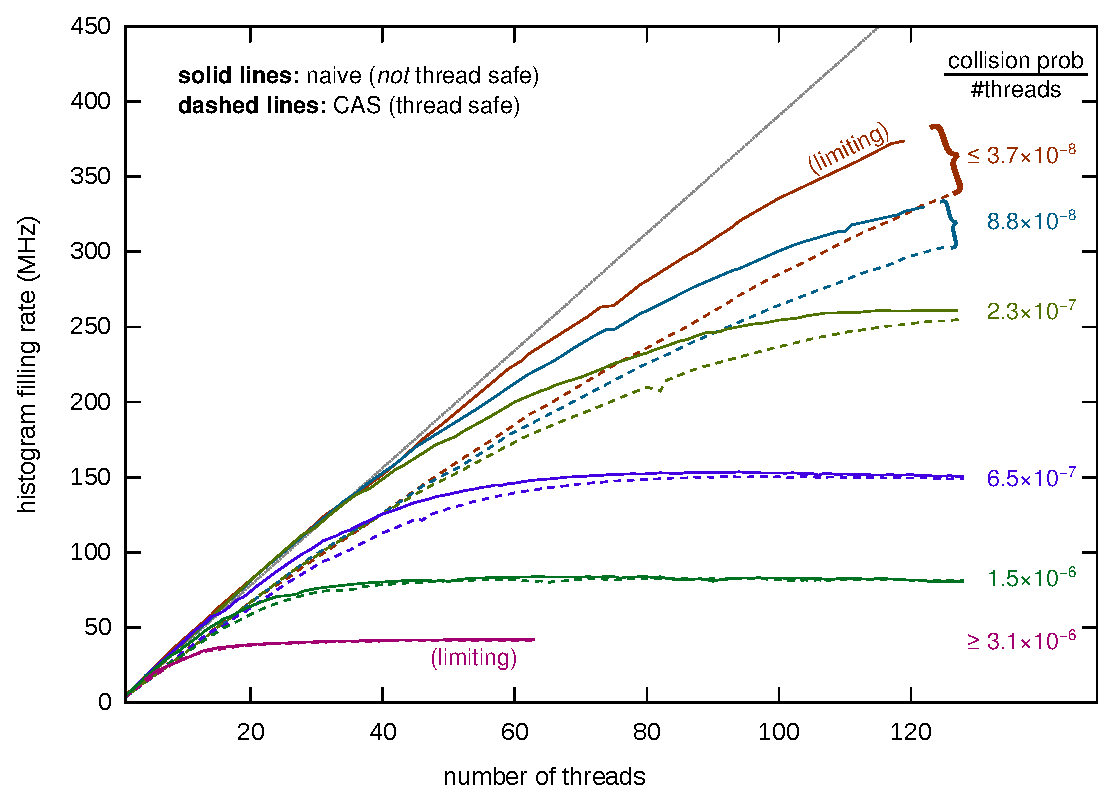
\includegraphics[width=\linewidth]{overlay.pdf}

\vspace{-4.3 cm}
\begin{uncoverenv}<2->
\hfill 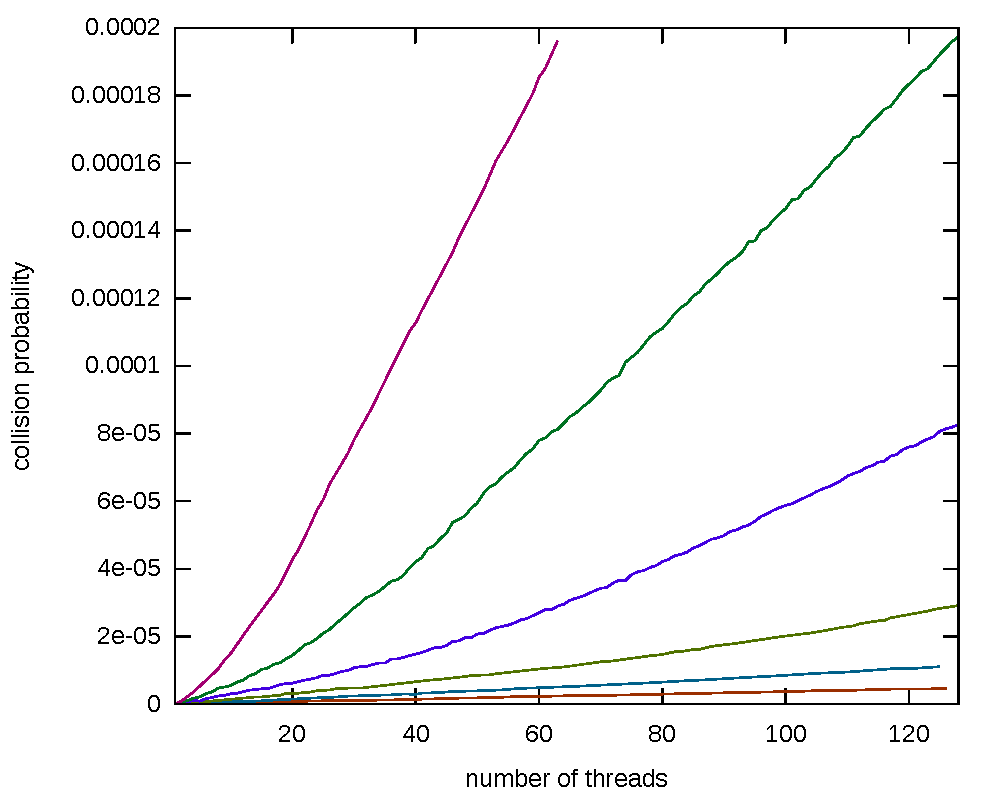
\includegraphics[width=0.55\linewidth]{prob.pdf}\hspace{-1 cm}
\end{uncoverenv}
\end{frame}

\begin{frame}{{\tt std::atomic} results}
\vspace{0.5 cm}
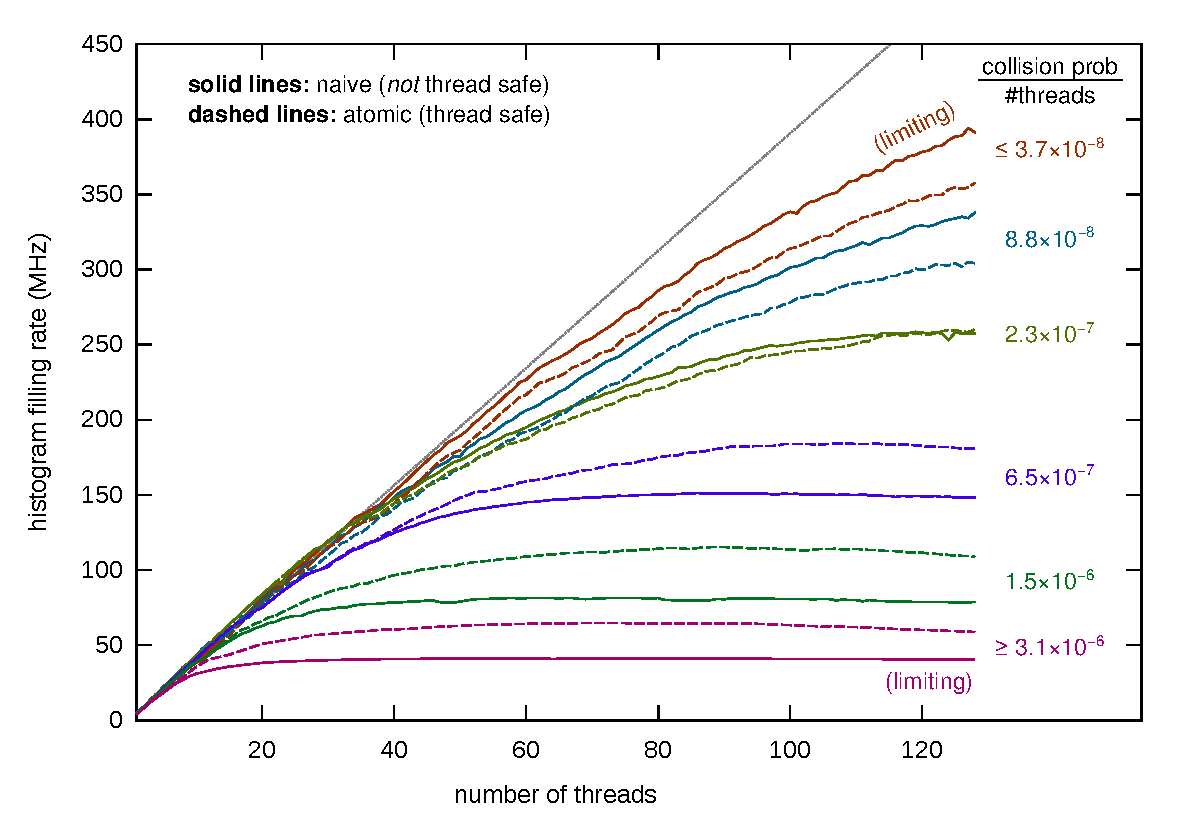
\includegraphics[width=\linewidth]{overlay2.pdf}
\end{frame}


\end{document}
